\documentclass[12pt, letterpaper]{article}

%Line Spacing
\usepackage{setspace}
\doublespacing

%Graphics
\usepackage{graphicx}

%Margins
\usepackage[margin=1in]{geometry}

%Citations
\usepackage[backend=biber,style=ieee,urldate=long]{biblatex}
\addbibresource{refs.bib}

\title{Passwordless Authentication}
\author{Zachary Thompson}

\begin{document}
\maketitle

\section{Executive Summary}

\newpage
\section{Introduction}
Passwordless authentication describes a collection of authentication methods which do not rely on the user remembering and entering a password in order to be authenticated.
Proponents of passwordless authentication argue it is both more convenient and more secure than traditional, password-based authentication.

This paper will look at the flaws of password based authentication and analyze whether passwordless authentication can address them.
It will describe various methods of passwordless authentication and discuss their benefits and drawbacks.

\newpage
\section{Discussion}
\subsection{The Problem With Passwords}
Password-based authentication has a number of flaws.
For one, passwords are prone to reuse.
It is difficult to remember dozens of unique passwords, so people end up using the one they already memorized over and over again.
According to a poll conducted by Google and Harris in 2019, 52\% of people reuse a password for multiple accounts and 13\% reused a password for all of their accounts \parencite{googleharris2019poll}.
If an attacker were to compromise one password, then there is a good chance they could use it to breach other accounts.

Another problem is that good passwords are difficult to memorize.
Good passwords are long and use different types of symbols.
Ideally, a password would be a long, randomly generated string of characters.
A password like that is hard enough to memorize for one website, let alone all of them.

Password managers help in this regard.
They are able to generate and store passwords for you.
This means that, assuming the password manager is used correctly, all of your passwords will be difficult to crack and will be unique. 
However, all of your passwords are now only as strong as your master password (and the security of your password manager).

Passwords are particularly vulnerable to any sort of attack which involves the attacker stealing the password.
A common example of this type of attack is phishing; the attacker tricks the user into entering their password by sending them a deceptive message.
Phishing was the most common type of cyber crime in 2020 and a password manager will not defend against this type of attack \parencite{fbi2020icr}.

Clearly passwords have a number of flaws which need to be addressed.
81\% of hacking-related security breaches in 2017 involved stolen or weak passwords, so there is plenty of reason to look for an alternative authentication method \parencite{verizon2017dbir}.

\subsection{A Solution: Get Rid of the Password}
Perhaps one way to eliminate the problems of passwords is to use some other form of authentication.
That is exactly what Microsoft allows you to do with their Authenticator app. 

\begin{figure}[ht]
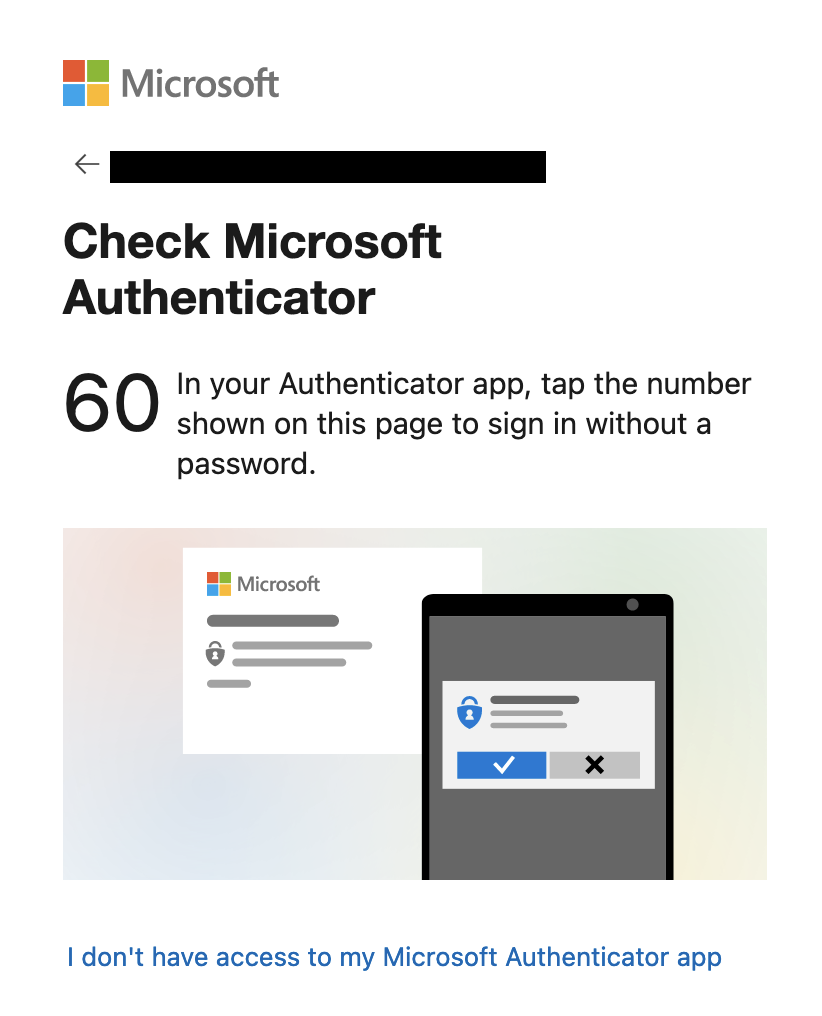
\includegraphics[width=0.5\textwidth]{mslogin.png}
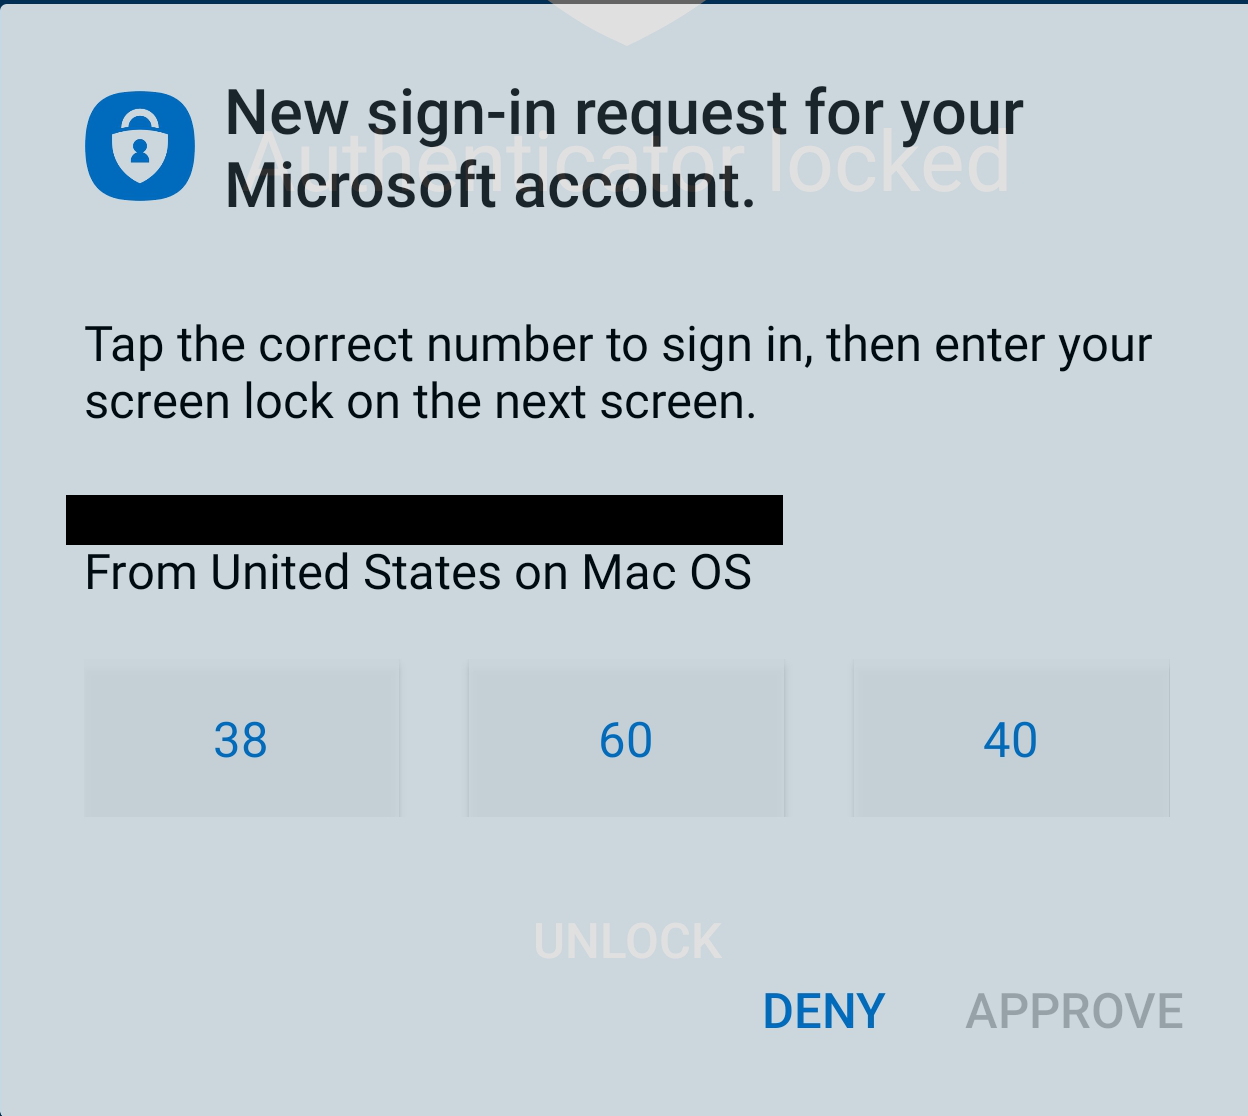
\includegraphics[width=0.5\textwidth]{authenticator.png}
\caption{Microsoft's Passwordless Authentication\label{msauth}}
\end{figure}

Figure \ref{msauth} shows what Microsoft's passwordless authentication is like.
Every time you login to your Microsoft account you will get a prompt on your phone which will ask you to select the same number that is displayed on the device you wish to log into.

\subsection{Account Recovery}
If the user is no longer able to access their authentication method, then there needs to be some form of account recovery so that the user can fix the issue.

\newpage
\section{Analysis and Recommendations}

\newpage
\section{Conclusion}

\printbibliography
\end{document}
